% define the type of document I want to make (article), set 12pt font and letter-sized paper
\documentclass[12pt, letterpaper]{article}

% the natbib package lets me use extra citation commands, authoryear sorts bibliography by author last name, then year of publication
\usepackage[authoryear]{natbib}
% the hyperref package lets me insert a hyperlink, and makes table of contents and references clickable
\usepackage{hyperref}
% graphicx allows....graphics
\usepackage{graphicx}
% letting LaTeX do line breaks easier so it doesn't complain about hboxes
\setlength{\emergencystretch}{5pt}


% enter the document environment to begin!
\begin{document}

% set the title
\title{Homework 4 - PHYS 5391}
% set author
\author{Elizabeth Vandegriff}
% set date as current date
\date{\today}

% make the above title/author/date visible
\maketitle
% leave the rest of the title page blank
\newpage
% create a table of contents based on the sections I define throughout the doc
\tableofcontents
% start sections on new page after table of contents
\newpage

\section{Weasels!}

Can you recreate the simple phrase ``METHINKS IT IS LIKE A WEASEL'' in Python by starting with a random string of characters? Randomly changing characters until you arrive at the target phrase has an extremely low probability of succeeding, but when the process is guided by a sort of natural selection acting on each ``generation'' of strings, this goal is easily achievable.

What this involves is defining the random starting string as generation 0, then creating a set number of ``offspring'' by randomly changing the characters at a certain percentage rate, or ``mutation'' rate. Whichever one of the offspring is closest to the target phrase becomes the new parent phrase in the first generation, and the cycle continues down generations until the target phrase is acquired.

I have created a function that can reproduce the intended phrase given a set generation size and mutation rate. For example, with a generation size of 100 and a mutation rate of 4\%, my weasel program can reach the target phrase in an average of ~80 generations; that is to say, the ``weasel convergence'' for a generation size of 100 and a mutation rate of 4\% is 80. I will use the term ``weasel convergence'' in the remainder of my description for brevity.

\section{How My Weasel Program Works}

My weasel program uses the string module to assemble the alphabet and the space character as the allowed list of characters to create the target phrase from. I use the random module to choose random characters from the allowed set until I have a string the same length as the target phrase. This string becomes the first parent string, generation zero.

I then enter a while loop that only exits when it has reached the target phrase. Within the while loop, I create each offspring by copying the parent string and looping through each letter to ``mutate'' it. I again use the random module to allow a specific mutation rate, specifying that if the random number generator falls in between 0 to the selected mutation rate, the letter will change. In my specific code, I chose to add another while loop that guarantees that the mutated character will \textbf{never} be the same as the original letter. I did this to ensure that the mutation rate is accurately represented in the algorithm.

After looping through the entire string, I add this offspring string to a list of offspring, and continue to create them until I have a full generation. I then cycle through the offspring and assign each one a score: one point for every character that matches the target phrase. I then take the string with the highest score and set that as my new parent string. Now, the whole cycle begins again, first with the while loop determining whether the target phrase has been achieved.

After many generations, the offspring string will finally match the target, the while loop exits, and the weasel convergence is printed to the screen.

Figure (\ref{fig:mean1000}) shows the mean weasel convergence of a single run, then 1000 runs of the program with fixed generation size at 100 and fixed mutation rate at 4\%.

\begin{figure}[!ht]
  \centering
  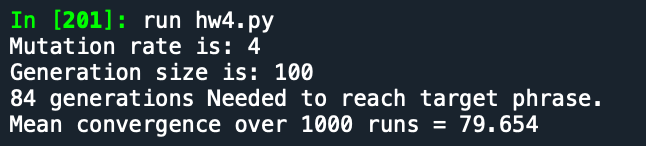
\includegraphics[width=12cm]{mean_1000_runs.png}
  \caption{Taking the mean weasel convergence over 1000 runs of the weasel program.}
  \label{fig:mean1000}
\end{figure}



\section{Exploring the Weasel Program}

So far I have only talked about my weasel program in the case of fixed generation size 100 and fixed mutation rate 4\%. But do these parameters affect the weasel convergence? What happens when I vary these parameters?

To answer these questions, I created a function to test either of the parameters in the weasel function within a specified range. This function enables me to run my weasel program thousands of times without me having to run and save results manually, which would take an extremely long time. I specify which variable to explore, the start and stop values for that variable, then how many times I would like to run the weasel program with each step before taking the average value. The function will then use the dictionary of the input values and the mean weasel convergence numbers for the entire range specified. Of course, this data is infinitely more valuable when plotted, so the function also plots the dictionary, with weasel convergence on the y-axis and either generation size or mutation rate on the x-axis. Figure (\ref{fig:varmut}) shows a plot made with my exploration function focused on the mutation rate.

\begin{figure}[!ht]
  \centering
  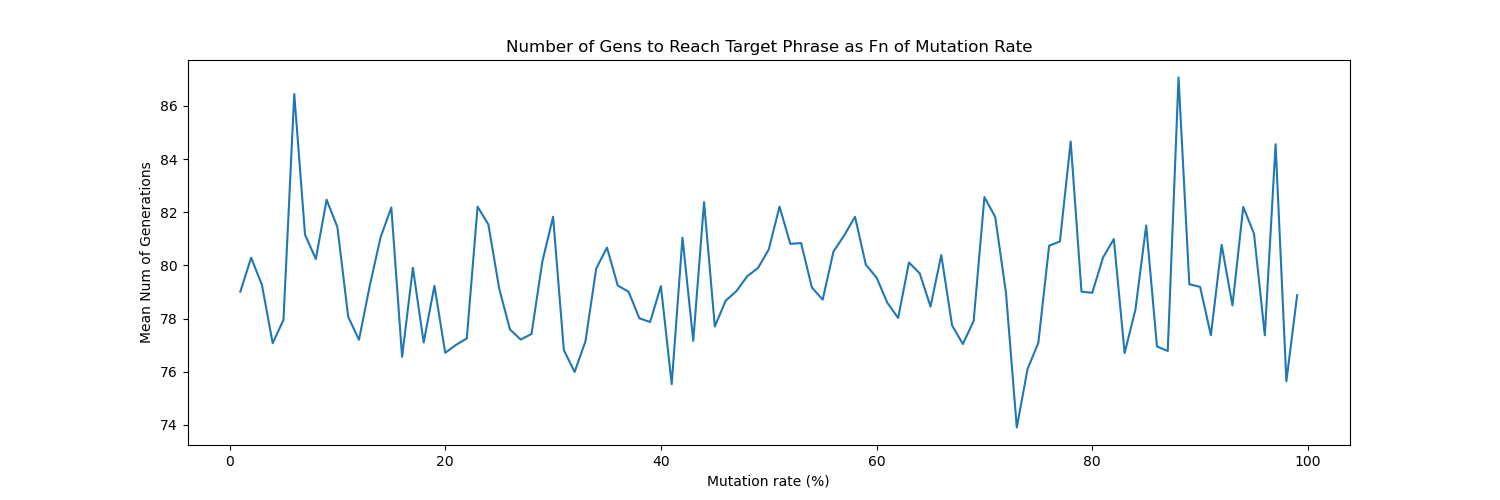
\includegraphics[width=12cm]{../plots/Mut_mean_100_1_to_100.png}
  \caption{Exploring weasel convergence as a function of mutation rate.}
  \label{fig:varmut}
\end{figure}


In Figure (\ref{fig:varmut}) there seems to be no clear correlation between the weasel convergence and mutation rate. This particular plot uses 100 runs to create the mean value at each mutation rate step. I decided to try using 1000 runs for the mean to see if anything changed. This is shown in Figure (\ref{fig:varmut1000}).

\begin{figure}[!ht]
  \centering
  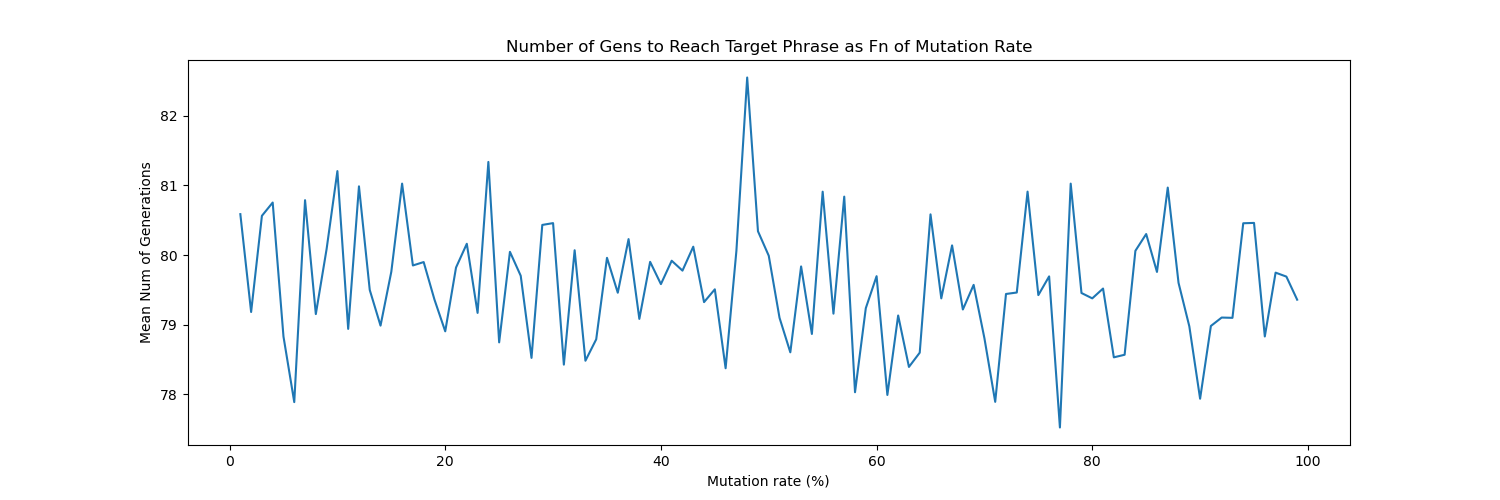
\includegraphics[width=12cm]{../plots/Mut_mean_1000_1_to_100.png}
  \caption{Exploring weasel convergence as a function of mutation rate, using 1000-run mean weasel convergences.}
  \label{fig:varmut1000}
\end{figure}

Clearly even with using more runs, there is no discernible correlation between the two variables.

Now we use the exploration function to look at generation size, shown in Figure (\ref{fig:vargen}). Clearly, the weasel convergence drops dramatically as generation size increases. I only ran the generation size variable with 100-run means, because the 1000-run means take many hours to complete, and I could already see the correlation perfectly well. I can conclude from this plot that as the generation size increases, the number of generations needed to reach the target phrase decreases.

\begin{figure}[!ht]
  \centering
  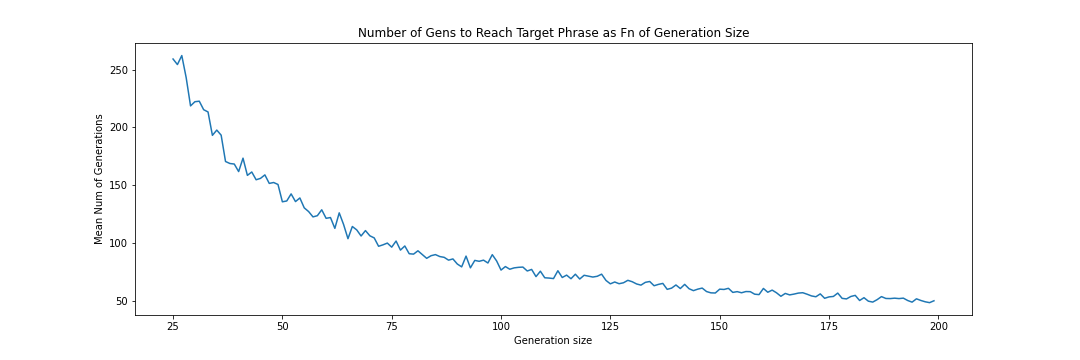
\includegraphics[width=12cm]{../plots/Gen_mean_100_25_to_200.png}
  \caption{Exploring weasel convergence as a function of generation size.}
  \label{fig:vargen}
\end{figure}



\section{Limitations}

In Figure (\ref{fig:vargen}), you may notice that I do not start the generation size below 25. There is a good reason for this; namely, for smaller and smaller generation sizes, the weasel convergence gets higher and higher. Eventually, the program does not converge at all! After running my program for single-digit generation sizes, I determined that a generation size of 9 is the smallest that can produce a result. The reason I did not plot 9 as the lower limit in Figure (\ref{fig:vargen}) is because the weasel convergence was so high (see Figure (\ref{fig:lowlim})) it would have obliterated the scale of the plot. 

\begin{figure}[!ht]
  \centering
  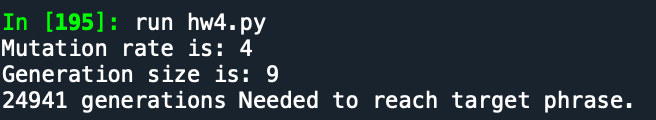
\includegraphics[width=12cm]{gen_size_9.png}
  \caption{Weasel convergence for the lowest possible generation size.}
  \label{fig:lowlim}
\end{figure}

My strategy overall was to minimize the use of for loops, to make the program run more quickly, and to streamline the process so that I would not need to manually run my weasel program to explore the two variables. This was achieved using my two functions, the weasel program itself and the variable exploring function, which both have sensible inputs, outputs, and capabilities for print statements (depending on whether you want to see the input and results on screen each time the weasel program is run). I thought of other possibilities that I did not explore because they would take much longer to implement. One such idea was to adjust the actual weasel code to stop mutating a character from generation to generation once it is the same as the target phrase, although I am not sure if this has any parallels to biology.


\end{document}
